\documentclass[12pt]{article}
%Gummi|065|=)
\usepackage{amsmath, amsfonts, amssymb}
\usepackage[margin=0.5in]{geometry}
\usepackage{xcolor}
\usepackage{graphicx}

\newcommand{\off}[1]{}
\DeclareMathSizes{20}{30}{20}{18}

\newcommand{\two }{\sqrt[3]{2}}
\newcommand{\four}{\sqrt[3]{4}}


\usepackage{tikz}

\title{the Schr\"{o}dinger Equation}
\author{John D Mangual}
\date{}
\begin{document}

\fontfamily{qag}\selectfont \fontsize{12.5}{15}\selectfont

\maketitle

\noindent When I opened up Quantum Mechanics by Enrico Fermi, I just expected just some kind of review.  These course notes are facisimile of a class at University of Chicago in 1954 written by one of the ``greats". \\ \\
There are some things that are unusual.  He opens with a \textbf{optics-mechanics} analogy:
\begin{center}
\begin{tabular}{l|l} 
mass point & wave packet \\ \hline  \\ 
trajectory & ray \\  \hline \\
velocity & group velocity \\ \hline  \\
??? & phase velocity \\  \hline \\
potential function & refractive index \\ \hline  \\
energy & frequency \\  \hline \\
\end{tabular}
\end{center}
Hopefully, if you've taken a quantum mechanics course, you may have heard of ``particle-wave duality" even if you can't qualify what it meant.  \\ \\
What is\dots \textbf{particle-wave duality}? 
\begin{center}
\begin{tabular}{lcl}
Trajectory &=& Ray \\ 
$\downarrow$ & & $\downarrow$ \\
from Maupertuis & & from Fermat \\ 
$\downarrow$ & & $\downarrow$ \\
$\int \sqrt{E - U}\, ds = min $ & & $\int \frac{ds}{v} = min$
\end{tabular}
\end{center}
He then proceeds to prove the Maupertuis and Fermat principles (of optics). \\
A beam of light ``searches for" the optimal path in one of two different ways:
\begin{itemize}
\item principle of least action
\item principle of least time
\end{itemize}
For clarification: $E$ is the total energy.  Maupertuis principle is \textbf{not} the principle of least action.
\begin{quotation}
is that the path followed by a physical system is the one of least ``length"
\end{quotation}
OK.  Maupertuis $ \neq $ Huygens, which is the one I really like. I will give a fake derivation

\newpage

\noindent First of all $v = \frac{ds}{dt}$.  Velocity is the derivative of time.  Therefore $\frac{ds}{v} = dt $, and in fact we should get time:
$$ T = \int \frac{ds}{v} $$
That was too easy.  Let's do the other one now.\footnote{Optics is not a field I now very well (in fact it's a special case of \textbf{electromagnetism}, yet Optics has been studied since Newton and Electromagnetism those equations are due to Maxwell.  I don't know a good analogue for \textit{refractive index})}  Let $U=0$ and $E = \frac{1}{2} m v^2$, and if we write:
$$  \int \sqrt{E} \, ds = \int \sqrt{\tfrac{1}{2}mv^2} \, ds =  \int v \, ds =
\int \frac{ds}{dt} ds = \int \left(\frac{ds}{dt}\right)^2 \, dt  = \int v^2 \, dt $$
and this should be zero for all possible $\delta v = 0$.  The first variation should be:
$$ \delta \int \sqrt{E} \, ds = \delta \int v^2 \, dt
= \int (v + \delta v)^2 \, dt - \int v^2 \, dt  = 2 \delta v \int v \, dt = \delta v \int ds  $$
And we have shown both Fermat and Mauperthuis lead to length minmization.  \\ \\
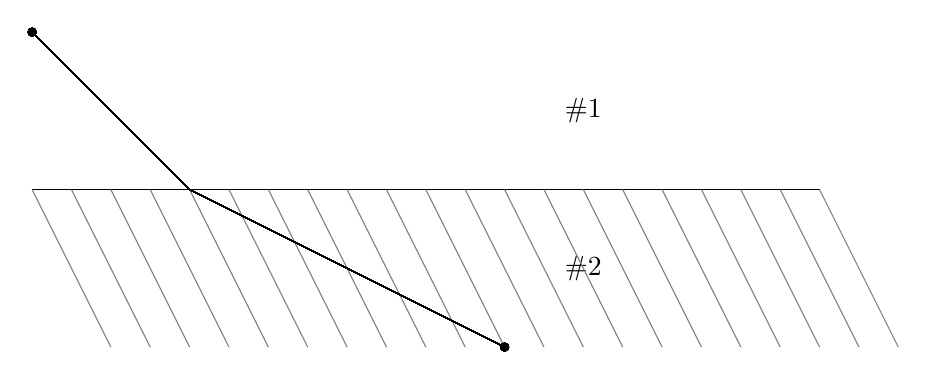
\begin{tikzpicture}
\node at (7, 1) {\#1};
\node at (7,-1) {\#2};
\draw (0,0)--(10,0);
\foreach \a in {0,...,20}{
\draw[color=black!50!white] (\a/2,0)--(\a/2+1,-2);
\draw (0,2)--(2,0)--(6,-2);
\draw[fill=black] (0,2) circle (0.05);
\draw[fill=black] (6,-2) circle (0.05);

}
\end{tikzpicture} \\ \\
This is the worst derivation ever.  Yet it reflects the equality of derivations we have in a typical Lagrangian mechanics textbook.  And likely, as must as Mr. Fermi had in mind.  \\ \\
We'll see his derivation wasn't much better, but at least he can get us to Schr\"{o}dinger.

\newpage

\noindent It's hard to know how to continue this because Fermi's development is just so far-fetched.  I'm a bit rusty, however:
$$ \mathbf{p} = m \mathbf{v} \hspace{0.125in}\text{ and }\hspace{0.125in} E = \frac{1}{2} m v^2 \hspace{0.25in}\text{ therefore }\hspace{0.25in} E = \frac{p^2}{2m}$$
In physics class, quantization is just a procedure for generating the Schr\"{o}dinger equations:
$$ \mathbf{p} = i\hbar \nabla \text{ and we just said }E = \frac{p^2}{2m} \text{ so that } - \frac{\hbar^2}{2m} \nabla^2 \psi = E \psi $$
and that is the free particle Schr\"{o}dinger equation.  And it's solutions are the standing waves:
$$ \psi(r, t) = A \, e^{ - \frac{1}{i\hbar}(\mathbf{p}\cdot \mathbf{r} -  E \, t)} $$
That's really well.  The reason we solve th wave equation in class is because it's the only differential equation we know how to solve. All other cases, have boundedness issues and well-posedness issues that have never been resolved. \\ \\
The other problem is that I learned quantum mechanics about 7 years ago in 2009 back in Califronia.  I left there on very bad terms and havn't been since 2012. 
$$ K_t(x,y) = K_t(x-y) = \frac{1}{\sqrt{2\pi i t}}e^{-\frac{i(x-y)^2}{2t}} \stackrel{t\to 0}{\longrightarrow} \delta (x-y)$$
The propagator is away of ``generating" the evolution -- how the wave function changes oer time.  My approach is neither
\begin{itemize}
\item rigorous enough for functional analysts
\item physically relevant enough for engineers
\item visual enough for geometers
\end{itemize}
There are people who make entire careers out of studying Laplacian operators on surfaces:
$$ \nabla^2 = \frac{\partial^2 }{\partial x^2 }
+ \frac{\partial^2 }{\partial y^2 }
+ \frac{\partial^2 }{\partial z^2 }$$
and here we specify we are doing the Laplacian on $\mathbb{R}^2$ (flat Euclidean space).\\ \\
Feynman uses the Lagrangian (instead of the Hamiltonian) for the Path integral:
$$ \text{Lagrangian} = \text{Potential}-\text{Kinetic} \hspace{1in} 
\text{Hamiltonian} = \text{Potential}+\text{Kinetic} $$
In the case of free particle $L = \frac{1}{2}mv^2$ so that the propagator is:
$$ K_0(b,a) = \lim_{\epsilon \to 0} \left( \frac{m}{2\pi i h \epsilon} \right)^{N/2} 
\times \int \dots \int \exp \left\{ \frac{im}{2\hbar\epsilon} \sum_{i=1}^N  (x_i - x_{i-1})\right\} dx_1 \dots dx_{N-1}$$
\newpage

\noindent and if you do the infinitely many Gaussian integrals: 
$$ K_0(b,a) = \sqrt{\frac{m}{2\pi i \hbar(t_b - t_a)}} \exp \left\{ \frac{ im (x_b - x_a)^2}{2\hbar (t_b - t_a)} \right\} $$
This answer makes sense.  The quantum free particle starts off concentrated at a point, and diffuses spreading out evenly in a circle.  \\ \\
We have now solved the free particle equation twice.  
\begin{itemize}
\item some kind of Gaussian diffusion
\item a wave
\end{itemize}
Maybe I'll conclude with my picture of the propagator. \\\\
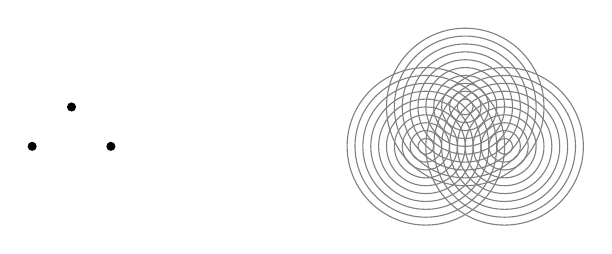
\begin{tikzpicture}

\draw[fill=black] (0,0) circle (0.05);
\draw[fill=black] (1,0) circle (0.05);
\draw[fill=black] (0.5,0.5) circle (0.05);

\begin{scope}[xshift=5cm]
\foreach \a in {1,...,10}{
	\draw[color=black!50!white] (0,0) circle (0.1*\a);
	\draw[color=black!50!white] (1,0) circle (0.1*\a);
	\draw[color=black!50!white] (0.5,0.5) circle (0.1*\a);
}

\end{scope}

\end{tikzpicture} \\ \\
Maybe can solve the Schr\"{o}dinger equation by taking minkowski sums of shapes:
\\\\
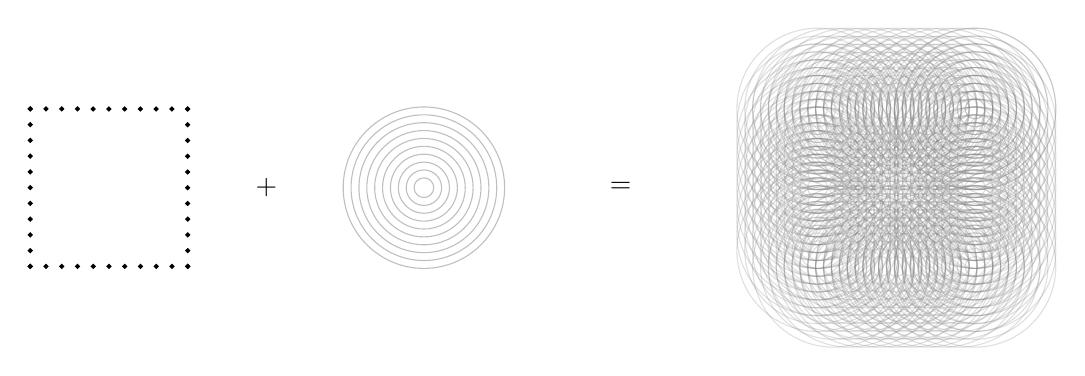
\begin{tikzpicture}

\foreach \a in {0,...,10}{
	\draw[fill=black] (0,0 + \a*0.2) circle (0.025);
	\draw[fill=black] (2,0 + \a*0.2) circle (0.025);
	\draw[fill=black] (0 + \a*0.2,0) circle (0.025);
	\draw[fill=black] (0 + \a*0.2,2) circle (0.025);
}


\node at (3,1) {+};

\foreach \b in {1,...,10}{
	\draw[color=black!50!white, opacity=0.5] (5,1) circle (0.025 + \b*0.1);
}

\node at (7.5,1) {=};

\begin{scope}[xshift=10cm]
\foreach \b in {1,...,10}{
	\foreach \a in {1,...,10}{
		\draw[color=black!50!white, opacity=0.25] (0,0 + \a*0.2) circle (0.025 + \b*0.1);
		\draw[color=black!50!white, opacity=0.25] (2,0 + \a*0.2) circle (0.025 + \b*0.1);
		\draw[color=black!50!white, opacity=0.25] (0 + \a*0.2,0) circle (0.025 + \b*0.1);
		\draw[color=black!50!white, opacity=0.25] (0 + \a*0.2,2) circle (0.025 + \b*0.1);
	}
}

\end{scope}

\end{tikzpicture}  \\ \\
and the wave function equation could read $\psi(t) = \psi(0) + K(t - 0)$ as shapes?

\newpage

\noindent \textbf{5/11} Vladimir Arnol'd was a world unto himself.  Let's pick three books:
\begin{itemize}
\item Mathematical Aspects of Classical Mechanics 
\item Catastrophe Theory
\item Contact Geometry and Wave Propagation
\end{itemize}
It's this last one that sets me off: really taking to heart that particle-wave duality is about particles and waves.  Who do I believe?  I would rather believe Enrico Fermi that Fermat, Huygens and the study of Newtonian optics could be related to the wave equation of Schr\"{o}dinger and Heisenberg.  \\ \\
It's exhausting to think this hard.  It's difficult to have a point of view when many clearly authoritative or expert sources point otherwise.  \\ \\
For starters: there is \textbf{sympletic geometry} (in even dimensions $\mathbb{R}^{2n}$) and \textbf{contact geometry} (in odd dimensions $\mathbb{R}^{2n+1}$).  None of my physics textbooks ( I not a physics major) discuss sympletic manifolds.  The most basic idea is position and momentum become interchangeable: 
$$\text{position} \leftrightarrow \text{momentum} \hspace{0.5in}\text{ so that }\hspace{0.5in} (\text{position}, \text{momentum}) \in \mathbb{R}^{2n} $$
and therefore physical degrees of freedom in mechanical systems come in pairs.  Yet, wave propagation seems to be about contact geometry. \\ \\
Whichever one you pick, modern symplectic geometry or contact geometry is unintelligible.  We will step back a couple of decades, as the most modern language is very much beyond my reach. 

\vfill

\begin{thebibliography}{}

\item Hansj\"{o}rg Geiges \textbf{Christiaan Huygens and Contact Geometry}

\item Richard Feynman.  \textbf{Quantum Mechanics and Path Integrals} Dover, 2010.

\item Enrico Fermi.  \textbf{Quantum Mechanics} University of Chicago Press, 1961.

\item David Tong \textbf{Quantum Field Theory} (Math Tripos, Part III)  \\ \texttt{http://www.damtp.cam.ac.uk/user/tong/qft/qft.pdf}

\item Matthew Schwartz \textbf{Quantum Field Theory} (class notes, Fall 2008) \\
\texttt{http://isites.harvard.edu/fs/docs/icb.topic521209.files/QFT-Schwartz.pdf}

\end{thebibliography}

\newpage

\noindent \textbf{7/01} Why the hell did I stop reading Fermi's book.  I went to the Strand bookstore yesterday and considered picking up a copy of Joyce's \textit{Ulysses}  insetad I was able to get his complete works.  This includes: Finnegan's Wake, Dubliners and others.  It's a literary tradition, I don't have too much experience with.\footnote{Neither reading, nor interacting with.} \\ \\
Fermi - an Italian - opens his book by comparing Netwton's equations for particles and the Wave equation describing a beam of light.\footnote{Wikipedia says, Huygens principle for optics is found in 1670's while Jean d'Alembert would ``discover" the wave equation by 1750.} All Quantum Mechanics textbooks open with the Schr\"{o}dinger equation, but nobody tells you why the damn thing occurs. \\ \\
Fermi gives an explantion of \textbf{why} particles behave like waves.  It's fantastical, it has gaps, it's starting point. Does anyone else write like that?  In 2 months I've found one hint:
\begin{quotation}
Symplectic geometry is a generalization of Hamiltonian mechanics to manifolds more
general than the cotangent bundle $T(Q)$ of some n-dimensional configuration space $Q$
\end{quotation}
These are from notes on a Part III course at Cambridge.\footnote{\texttt{http://www.damtp.cam.ac.uk/research/gr/members/gibbons/gwgPartIII\_{}DGeometry2011-5.pdf}} The cotangent bundle here is simply the pairing of the position and the momentum:
$$ (x, p)  = ( x, \frac{dx}{dt}) \in T^\ast (\mathbb{R}^2) $$
And today in the early 21st centry, symplectic geometry goes totally berzerk using all sorts of functors and categories and it looks like a big mess.  And my question is how did the wave equation do all of that? \\ \\
No answers and that's why this one has been so quiet.

\vfill 

\begin{thebibliography}{}

\item Mich\'{e}le Audin.  \textbf{Morse Theory and Floer Homology} Springer, 2014.

\end{thebibliography}


\end{document}